\documentclass{article}

\usepackage{amsmath}
\usepackage{graphicx}
\usepackage{wrapfig}
\usepackage[margin=.9in]{geometry}

\begin{document}
\title{Project 1 Design Doc}
\author{Stern Huang (sh972) \& Colin Huang (ch645)}
\maketitle
\section{Introduction}
This is a design document for the \textbf{Project 2: Fully Pipelined MIPS} of CS 3410 (Spring 2014). In it, we will be describing our mini processor is implemented. This document is intended for the instructors of CS 3410 to read and and better understand how our circuits work. \\

\section{Overview}
\begin{center}
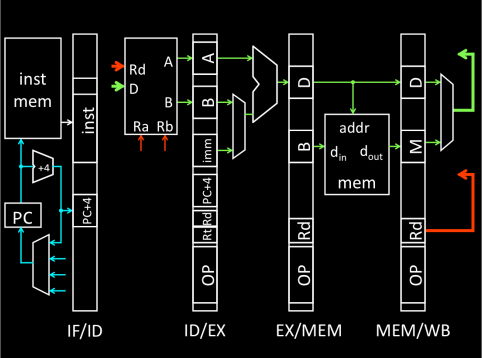
\includegraphics[scale=1.3]{pipeline.png} \\
Figure 1: Pipeline
\end{center}
\newpage
Creating the processor will consist of implementing 5 major pieces: \vspace{-3mm}\\ 
\begin{wrapfigure}{r}{0.35\textwidth}
\vspace{-1.7cm}
\begin{center}
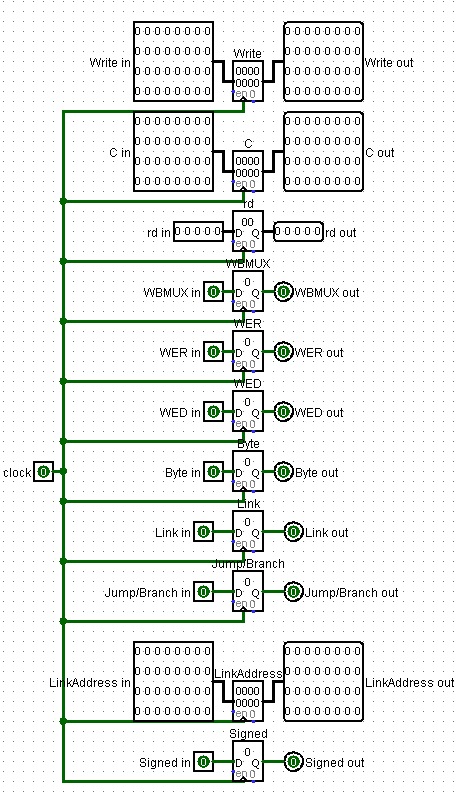
\includegraphics[scale=0.55]{isolator34.png} \\
Figure 2: Execute-Memory Isolator
\end{center}
\vspace{-1.5cm}
\end{wrapfigure}
\vspace{-0.7cm}
\begin{enumerate}
\item
\textbf{Pipeline Structure}: The implementation of a pipeline (Figure 1) requires the use of a clock as well as several registers to move data between different sections of the pipeline. We will refer to these as "\textbf{Isolators}" (Figure 2), as they isolate the various stages. Pipelining will be further explained in \textbf{Section 2.1}.

\item
\textbf{Decoding}: We must decode an instruction given by the Program ROM. This will tell the the register and the memory when to write, and the ALU what operation to perform. Various other bits will be outputted as well, which will be further explained in \textbf{Section 4}.

\item
\textbf{Execution}: The instructions that must be implemented are far more complicated than what a simple ALU is capable of. In order to carry out those instructions, we will create a larger Execute circuit, in which we use the ALU to perform specific operations. The Execute circuit will be further explained in \textbf{Section 5}.

\item
\textbf{Memory and Writeback}: After Execution, we will have to direct the computed value to where it needs to be used. This is usually the Memory or Writeback stage, but is also sometimes the Fetch stage. The Memory and Writeback implementation will be futher explained in \textbf{Section 6 and 7}.

\item
\textbf{Testing}: In order to test the functionality of our processor, we will write a program using the MIPS language and input it into the ROM. If the result is the expected result, we can conclude that our implementation of the processor is correct.
\end{enumerate}

\subsection{Circuit Diagram}
\begin{center}
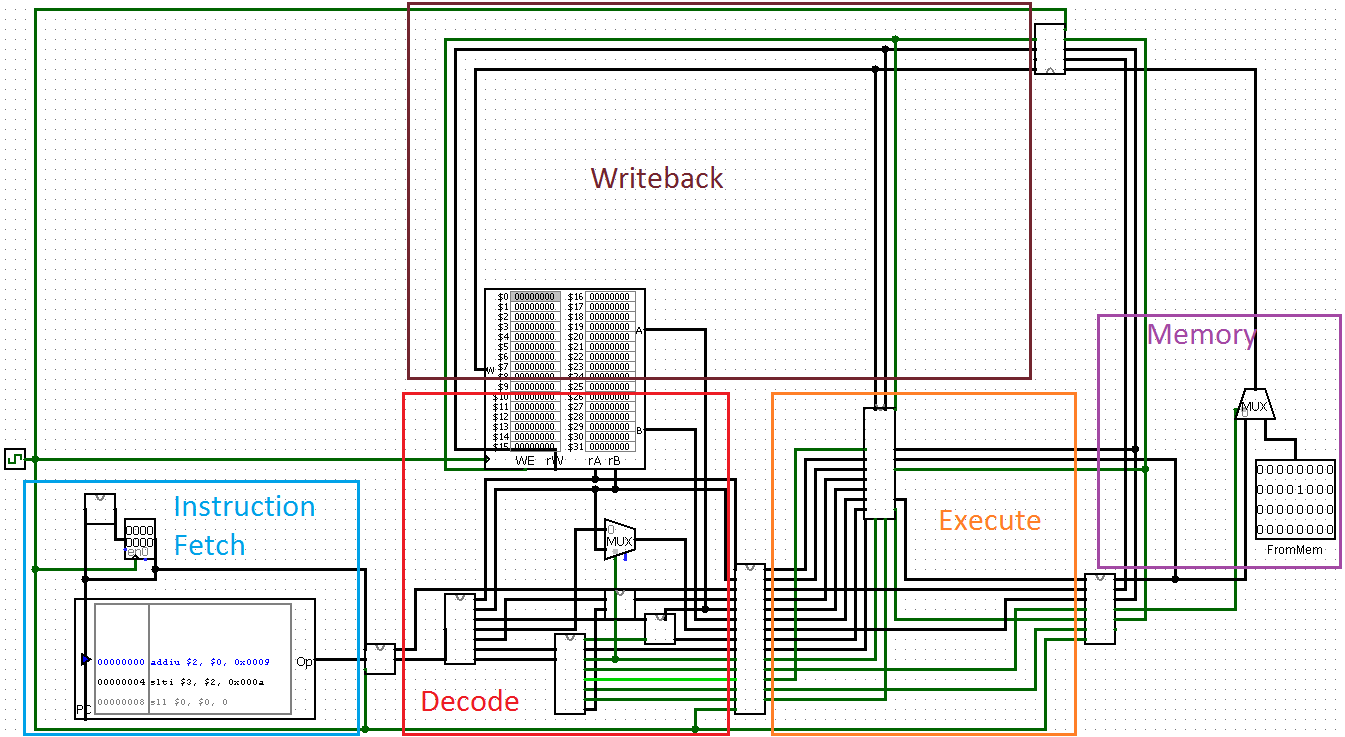
\includegraphics[scale=0.4]{Overview.png} \\
Figure 3: MIPS32 Circuit
\end{center}
The processor pipeline consists of 5 parts: \textbf{Instruction Fetch}, \textbf{Decode}, \textbf{Execute}, \textbf{Memory}, and \textbf{Writeback}. The clock on the far left determines when the data from one stage is transmitted to the next. This is done by the use of what we call \textbf{isolators}, which are simply a collections of registers that update on the rising edge of the clock. 

\section{The Fetch Stage}
The Fetch Stage is where the program instruction is extracted from the ROM. 
\subsection{Circuit Diagram}
\begin{wrapfigure}{r}{0.35\textwidth}
\vspace{-1.7cm}
\begin{center}
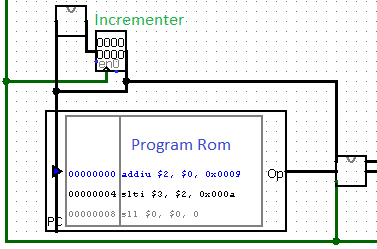
\includegraphics[scale=0.8]{Fetch.png} \\
Figure 4: Fetch
\end{center}
\vspace{-1.2cm}
\end{wrapfigure}
The Fetch stage has three main components: the \textbf{MIPS Program ROM},the \textbf{Incrementer} and the \textbf{Branching Circuit}. The MIPS Program ROM outputs 32-bit instruction codes depending on the inputted \textbf{program counter (PC)} to the isolator on the right. \\
The starting value of PC for any program is 0. Each subsequent instruction has PC 4 greater than that of the previous instruction. The incrementer will add 4 to the PC and store the result into the adjacent register on each clock tick. The register, however, is disabled when we must stall because of loading. \\
The branching circuit will usually output PC+4, as given by the incrementer. While branching, however, we it will instead output the jump or branch address. \\
The PC and the instruction code will be stored in the isolator to be used in the Decode stage. \\

\subsubsection{Submodule A: Incrementer}
\begin{wrapfigure}{r}{0.5\textwidth}
\vspace{-1.4cm}
\begin{center}
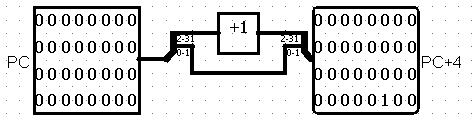
\includegraphics[width=0.5\textwidth]{Incrementer.png}\\
Figure 5: Incrementer
\end{center}
\vspace{-13mm}
\end{wrapfigure}
Figure 5 on the right is the Incrementer. We simply take the bits 2 through 32 and increase the value by 1. After appending back on the two least significant bits, we essentially have added 4 to the PC.

\subsubsection{Submodule B: Branch Circuit}
\begin{wrapfigure}{r}{0.4\textwidth}
\vspace{-1cm}
\begin{center}
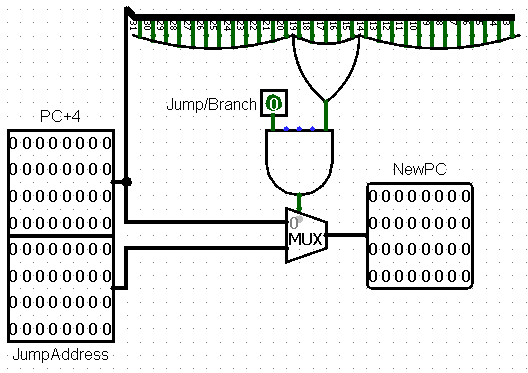
\includegraphics[width=0.4\textwidth]{FetchBranch.png} \\
Figure 6: Branching Circuit
\end{center}
\vspace{-1cm}
\end{wrapfigure}
Figure 6 is the branching circuit. It takes the inputs \

\subsection{Correctness Constraints}
The functional requirements for the circuit is as follows:
\begin{itemize}
\item
The \textbf{MIPS Program Rom} is correctly implemented, and has a valid Program inputted. In other words, the ROM must take a 32 bit Program Counter input, and output a 32 bit instruction code. 
\end{itemize}
While not every MIPS instruction has been implemented, it will not change the functionality of the fetch stage. 

\subsection{Testing}
In order to verify the functional correctness of this module, we simply load a text file with MIPS instructions into the Program ROM and turn on the clock. We expect the value of \textbf{PC} to increase by 4 every clock tick. We should also observe the instructions slowly scrolling through in the ROM.

\section{Instruction Decode}
\begin{wrapfigure}{r}{0.45\textwidth}
\vspace{-2.1cm}
\begin{center}
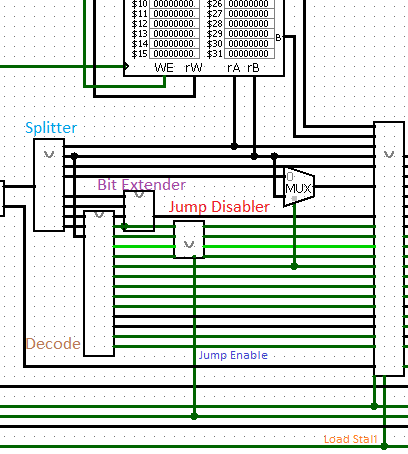
\includegraphics[scale=0.75]{DecodeOut.png} \\
Figure 6: Decode
\end{center}
\vspace{-4cm}
\end{wrapfigure}
Instruction Decode is where the 32 bit instruction is read and decoded. Here we will figure out exactly the instruction is going to do, determining key values such as write enable and select bits of multiplexors to be used in later parts of the pipeline. 

\subsection{Circuit Diagram}
The decode circuit takes the PC and instruction code from the Fetch-Decode Isolator. The instruction code is then used to compute numerous values. 

\newpage
The decode circuit consists of 3 main components: 
\begin{enumerate}
\item
In the \textbf{splitter}, the instruction code is broken into more useful pieces.

\item
The \textbf{register} uses two of the register addresses from the splitter, reads out of those registers, and inputs them into the next isolator.

\item
The \textbf{decode} unit takes the first and last 6 bits of the instruction code, and computes various values necessary for execution, and passes them to the next isolator. 
\end{enumerate}
As seen in the diagram, there are still minor circuits. I will briefly explain what each one does:
\begin{itemize}
\item
The MUX will determine which register we will write back to. In R-type instructions, the write-back register address is located in bits 11 to 15. However, in I type instructions, the write-back register address is located in bits 16-20. This MUX will choose between the two.

\item
The circuit directly under the MUX bit extends the 16-bit immediate value for I type instructions to the desired 32-bit value. The method of extension is determined by the decode unit.

\item
The circuit to the bottom right of the extender determines the shift amount that will be used in execute. The shift amount can either be bits 6 to 10 of the instruction code or the least significant 5 digits of a register. 
\end{itemize}

\subsubsection{Submodule A: Splitter}
\begin{wrapfigure}{r}{0.4\textwidth}
\vspace{-1.3cm}
\begin{center}
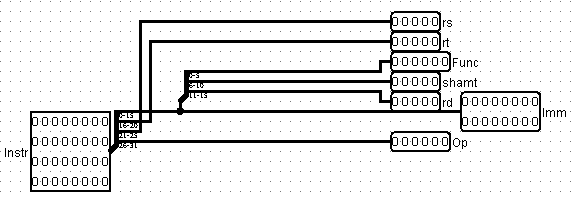
\includegraphics[scale=0.6]{Split.png} \\
Figure 7: Split
\end{center}
\end{wrapfigure}
Here, we can see the splitter break up the instruction code into several more useful pieces. Bits 0 to 15 make up the \textbf{immediate code}, which will be used in I type instructions. These 16 bits are then split into \textbf{function code}, \textbf{shift amount}, and \textbf{rd} which will be used in R type instructions. We will also have \textbf{Op} (bits 26 to 31) to determine the operation, and \textbf{rt} (bits 16 to 20) and \textbf{rs} (bits 21 to 25), the register addresses to be used.

\subsubsection{Submodule B: Decode}
The following table shows the desired outputs of each instruction:
\small
\begin{center}
\begin{tabular}{|c|c|c|c|c|c|c|c|c|} \hline
& \textbf{ALU} & \textbf{MUX 1} & \textbf{MUX 2} & \textbf{Write} & \textbf{Write} & \textbf{Shift} && \\
\textbf{Instruction} & \textbf{code} & \textbf{(Execute)} & \textbf{(Writeback)} & \textbf{Enable 1} & \textbf{Enable 2} & \textbf{Selector} & \textbf{Signed} & \textbf{Extend}\\ \hline
ADDIU & 001x & 1 & 0 & 1 & 0 &&&10\\ \hline
ANDI & 1000 & 1 & 0 & 1 & 0 &&&00\\ \hline
ORI & 1010 & 1 & 0 & 1 & 0 &&&00\\ \hline
XORI & 1100 & 1 & 0 & 1 & 0 &&&00\\ \hline
SLTI & 1111 & 1 & 0 & 1 & 0 &&1&10\\ \hline
SLTIU & 1111 & 1 & 0 & 1 & 0 &&0&10\\ \hline
ADDU & 001x & 0 & 0 & 1 & 0 &&&\\ \hline
SUBU & 011x & 0 & 0 & 1 & 0 &&&\\ \hline
AND & 1000 & 0 & 0 & 1 & 0 &&&\\ \hline 
OR & 1010 & 0 & 0 & 1 & 0 &&&\\ \hline
XOR & 1100 & 0 & 0 & 1 & 0 &&&\\ \hline
NOR & 1110 & 0 & 0 & 1 & 0 &&&\\ \hline
SLT & 1111 & 0 & 0 & 1 & 0 &&1&\\ \hline
SLTU & 1111 & 0 & 0 & 1 & 0 &&0&\\ \hline
MOVN & 1011 & 0 & 0 & 1 & 0 &&&\\ \hline
MOVZ & 1001 & 0 & 0 & 1 & 0 &&&\\ \hline
SLL & 000x & 0 & 0 & 1 & 0 & 0&&\\ \hline
SRL & 0100 & 0 & 0 & 1 & 0 & 0&&\\ \hline
SRA & 0101 & 0 & 0 & 1 & 0 & 0&&\\ \hline
SLLV & 000x & 0 & 0 & 1 & 0 & 1&&\\ \hline
SRLV & 0100 & 0 & 0 & 1 & 0 & 1&&\\ \hline
SRAV & 0101 & 0 & 0 & 1 & 0 & 1&&\\ \hline
LUI & 001x & 1 & 0 & 1 & 0 &&&01\\ \hline
J & xxxx & 1 & 0 & 0 & 0 &&&x1 \\ \hline
JR & xxxx & 0 & 0 & 0 & 0 &&& \\ \hline
JAL & xxxx & 1 & 0 & 1 & 0 &&&x1 \\ \hline
JALR & xxxx & 0 & 0 & 1 & 0 &&& \\ \hline
BEQ & 001x & 1 & 0 & 0 & 0 &&&10 \\ \hline
BNE & 001x & 1 & 0 & 0 & 0 &&&10 \\ \hline
BLEZ& 001x & 1 & 0 & 0 & 0 &&&10 \\ \hline
BGTZ& 001x & 1 & 0 & 0 & 0 &&&10 \\ \hline
BLTZ& 001x & 1 & 0 & 0 & 0 &&&10 \\ \hline
BGEZ& 001x & 1 & 0 & 0 & 0 &&&10 \\ \hline
LW & 001X & 1 & 1 & 0 & 1 &&& 10 \\ \hline
LB & 001X & 1 & 1 & 0 & 1 &&& 10 \\ \hline
LBU & 001X & 1 & 0 & 0 & 0 &&& 10 \\ \hline
SW & 001X & 1 & 0 & 0 & 0 &&& 10 \\ \hline
SB & 001X & 1 & 0 & 0 & 0 &&& 10 \\ \hline
\end{tabular} \vspace{2mm}\\
For the following table, the values for Instructions of Project 1 are all set to 0.
\begin{tabular}{|c|c|c|c|c|c|c|} \hline
& \textbf{Load/Store} & \textbf{Jump/Branch} && \textbf{Comp} & & \\ 
\textbf{Instruction} & \textbf{Byte} & \textbf{Enable} & \textbf{Link} & \textbf{Code} & \textbf{Branch} & \textbf{R Jump} \\ \hline
J &0& 1 & 0 & 000 & 0 & 0 \\ \hline
JR &0& 1 & 0 & 000 & 0 & 1 \\ \hline
JAL &0& 1 & 1 & 000 & 0 & 0 \\ \hline
JALR &0& 1 & 1 & 000 & 0 & 1 \\ \hline
BEQ &0& 1 & 0 & 010 & 1 & 0 \\ \hline
BNE &0& 1 & 0 & 011 & 1 & 0 \\ \hline
BLEZ &0& 1 & 0 & 100 & 1 & 0 \\ \hline
BGTZ &0& 1 & 0 & 111 & 1 & 0 \\ \hline
BLTZ &0& 1 & 0 & 101 & 1 & 0 \\ \hline
BGEZ &0& 1 & 0 & 110 & 1 & 0 \\ \hline
LW & 0 & 0 & 0  &000& 0&0 \\ \hline
LB & 1 & 0 & 0  &000& 0&0 \\ \hline
LBU & 1 & 0 & 0  &000& 0&0 \\ \hline
SW & 0 & 0 & 0  &000& 0&0 \\ \hline
SB & 1 & 0 & 0 &000& 0&0 \\ \hline
\end{tabular}
\end{center}
\normalsize
Any x's or missing fields mean that there is no preference between 0's and 1's. Notable variables include:
\begin{enumerate}
\item
\textbf{MUX 1}: This MUX select bit determines whether or not we are using an immediate value within Execute.

\item
\textbf{MUX 2}: This MUX select bit determines whether we are writing to the register from the ALU or from Memory.

\item
\textbf{Write Enable 1}: This determines whether or not we are writing to the register.

\item
\textbf{Write Enable 2}: This determines whether or not we are writing to Memory.

\item
\textbf{Shift Selector}: This bit determines whether the shift amount is from a register or from the 32 bit instruction code. (1 for register, 0 for instruction code)

\item
\textbf{Signed}: This bit determines whether the Less Than comparison considers the integers as signed or unsigned. (1 for signed, 0 for unsigned)

\item
\textbf{Extend}: This two bit code determines how the immediate value will be extended. Bit 1 determines whether we or sign extending or zero extending on the left. Then, bit 0 determines whether or not we must shifting the extended \textit{immediate} by 16 digits.

\end{enumerate}

\begin{wrapfigure}{r}{0.6\textwidth}
\vspace{-1cm}
\begin{center}
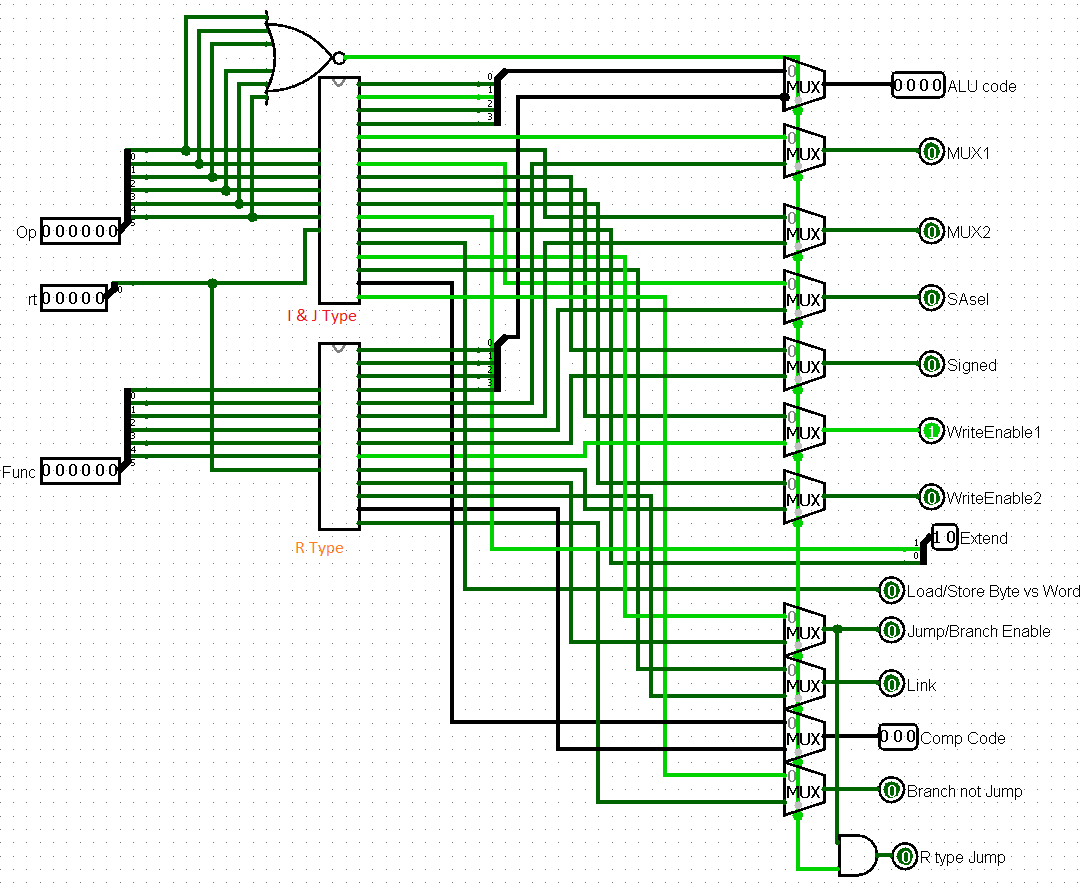
\includegraphics[scale=0.7]{Decoder.png} \\
Figure 8: Decode (subcircuit)
\end{center}
\vspace{-1.3cm}
\end{wrapfigure}
\noindent Figure 8 shows the Decode subcircuit. This is done in two major parts:
\begin{enumerate}
\item
For \textbf{I and J type instructions}, the operation is decided just by \textbf{opcode} (bits 26 to 31). Combinational analysis is then used on these 6 bits to determine output values.

\item
For \textbf{R type instructions}, \textbf{opcode} will be 000000, and the operation will be determined \textbf{function code} (bits 0 to 5). Once again, we use combinational analysis to determine outputs.
\end{enumerate}
The XNOR gate in the circuit determines whether the instruction is R type or I/J type. The resulting bit is then used as the select bit for the multiplexors at the end. Because R type instructions have no immediate value, we simply output the value for \textbf{Extend} from the I and J type combinational analysis circuit.

\subsection{Correctness Constraints}
The functional requirements for this circuit are as follows:
\begin{itemize}
\item
The operation desired must be within this project's scope. The implemented instructions are: \textbf{ADDIU}, \textbf{ANDI}, \textbf{ORI}, \textbf{XORI}, \textbf{SLTI}, \textbf{SLTIU}, \textbf{ADDU}, \textbf{SUBU}, \textbf{AND}, \textbf{OR}, \textbf{XOR}, \textbf{NOR}, \textbf{SLT}, \textbf{SLTU}, \textbf{MOVN}, \textbf{MOVZ}, \textbf{SLL}, \textbf{SRL}, \textbf{SRA}, \textbf{SLLV}, \textbf{SRLV}, \textbf{SRAV}, and \textbf{LUI}.

\item
While it is not used yet, the value of \textbf{PC} must be a multiple of 4. This is vital when implementing jumps and branches in the future.
\end{itemize}

\subsection{Testing}
To verify the functional correctness of this module, we can simply input 32 bit instruction codes, and check if our outputs are as expected. However, there are far too many possible combinations of 32 bit codes to test. Thus, it is more optimal for us to check if each subcircuit is correctly implemented. \\

\noindent The subcircuit \textbf{Split} is trivial, as it does not involve any logic gates. \\

\noindent The subcircuit \textbf{Decode} can be checked by manually inputting each implemented function's \textbf{opcode} and/or \textbf{function code}, and seeing if the outputs are consistent with the ones on the table. 

\section{Execute}
\begin{wrapfigure}{r}{0.4\textwidth}
\vspace{-2.1cm}
\begin{center}
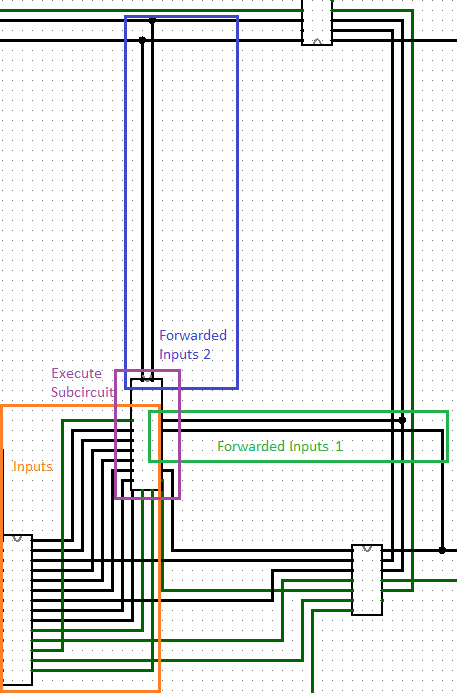
\includegraphics[width=6cm]{ALU.png} \\
Figure 9: Execute
\end{center}
\vspace{-2.5cm}
\end{wrapfigure}
The Execute stage is where most of the computation within an instruction occurs.
\subsection{Circuit Diagram}

Our Execute stage is all condensed into a big Execute subcircuit, that does the computing, (with additional lower level circuits within the subcircuit) and a smaller subcircuit that aids in stalling. The Execute subcircuit gets its inputs mainly from the ID/EX registers but also from the EX/MEM and MEM/WB registers for use in the forwarding unit. The four outputs of the subcircuit is the main output C, the Write Enable for the Register File (which is conditional in the MOV instructions), a Jump variable, indicating whether or not we branch, and an output for Store functions. 

The Execute subcircuit has many subcircuits of its own. For each of the main inputs, A and B, with respective register addresses rs and rt, there is a forwarding unit that resolves data hazard issues that are present in this Mini-Mips processor. There is a multiplexor for B that chooses between B and the immediate. There are special sections that implement commands whose outputs do not come from the ALU. These commands include SLT, SLTI, SLTIU, and SLTU; MOVZ and MOVN; jumps and branches; and SW and SB. 
\vspace{5mm}
\begin{center}
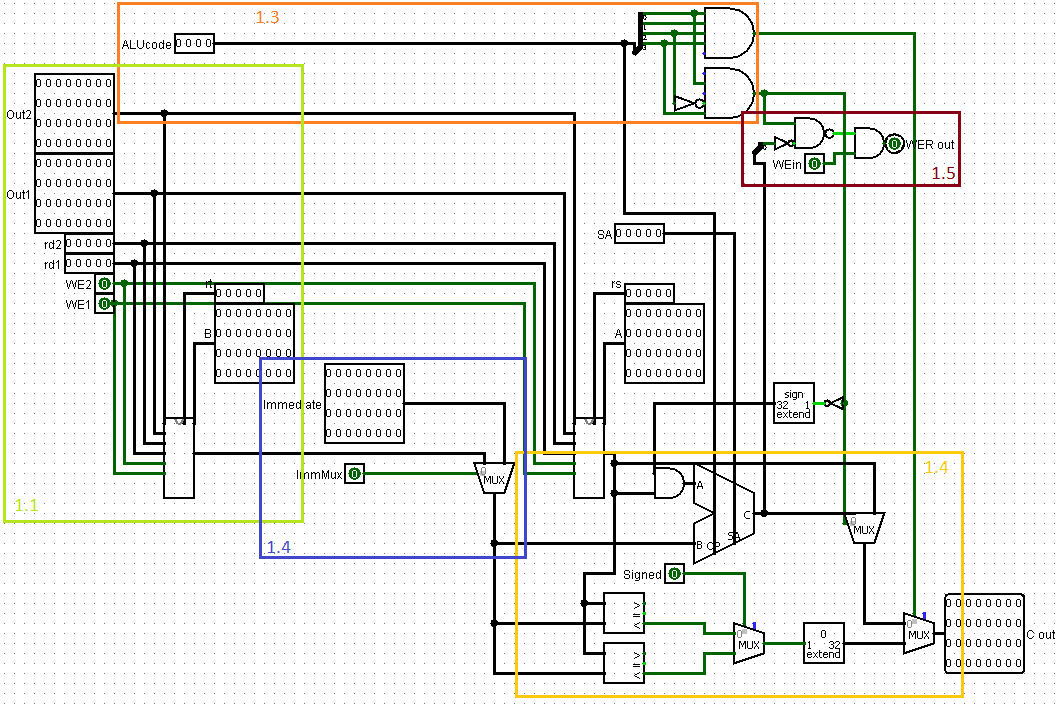
\includegraphics[width=15cm]{EXOVER.png} \\
Figure 10: Execute (Refer to this diagram for many of the subcomponents)
\end{center}

\subsubsection{General Purpose ALU}
The ALU (1.3) provides us the output for many of the simpler commands, and also provides us some intermediate outputs for the more specialized commands. Inputs A and B are determined by the specified command, but here we take them as given. We get the Op Code for the ALU as an input (1.1), and the SA is determined in a subcircuit (1.2), depending on whether or not the shift command was variable. 

\subsubsection{Forwarding Unit}
\begin{wrapfigure}{r}{0.27\textwidth}
\vspace{-1.5cm}
\begin{center}
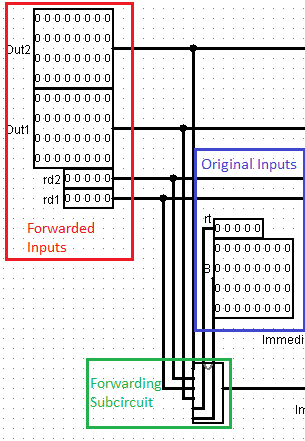
\includegraphics[scale=0.6]{Forward1.png} \\
Figure 11: Forward
\end{center}
\vspace{-5cm}
\end{wrapfigure}
This part of the circuit compares the register address (rs) of a main input (Out0) with the write destinations of the instruction in the next stage (rd1) and the stage after that (rd2). Out1 and Out2 are to be written in those destinations respectively. The write enable bits from those stages need to be included as well. The Forwarding Unit takes these 8 inputs and chooses one of the 3 32-bit outputs Out0, Out1, Out2. Figure 11 shows the layout of the Forwarding Unit and its inputs in the Execute circuit.

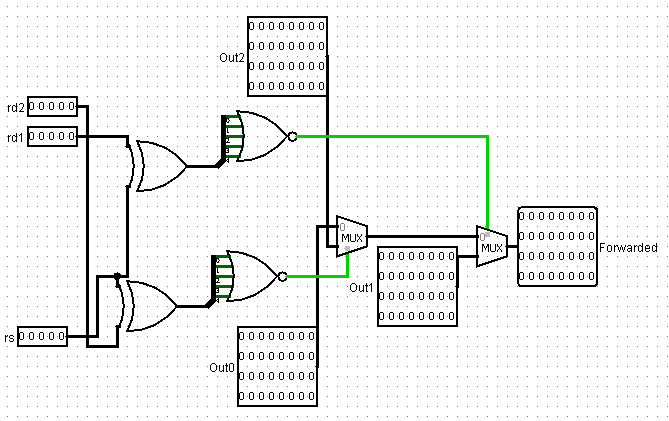
\includegraphics[scale=0.65]{Forward2.png}

\hspace{1.5cm}Figure 12: Forward (subcircuit) \\

\noindent The Forwarding Unit compares the register addresses using an XOR and a NOR gate, to get a multiplexor selector, that is, if the register addresses are equal, we get 1, and otherwise 0. This is ANDed with a write enable bit. This is done for each rs and rd1, and rs and rd2. We first choose between Out0 and Out2 by comparing rs and rd2, then the selected and Out1 by comparing rs and rd1. This process automatically gives Out1 higher priority than Out2; if all of rs, rd1, and rd2 are equal, Out1 will be chosen over Out2. 

\subsubsection{Immediate MUX}
\begin{wrapfigure}{r}{0.3\textwidth}
\vspace{-1.8cm}
\begin{center}
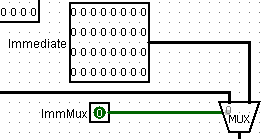
\includegraphics[scale=0.8]{Immediate.png}\\
Figure 13: Immediate MUX
\end{center}
\vspace{-1cm}
\end{wrapfigure}
This small section of the Execute circuit just chooses between Immediate and the second main input B. The Immediate is already bit extended to 32 bits, and our Decoder gives us a multiplexor selector bit ImmMux that we use here. 


\subsubsection{Special Command Determination}
\begin{center}
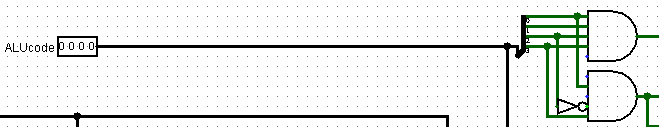
\includegraphics[scale = 0.9]{Code.png} \\
Figure 14: Special Commands
\end{center}
These 2 and gates explictly look for certain ALU Op codes. The Op code 1111 identifies the command as one of the SLT commands while the Op code 1x01 identifies the command as MOVN or MOVZ. We use these bits specially for executing these commands correctly in other parts of the circuit.

\subsubsection{Outputs}
\begin{wrapfigure}{r}{0.65\textwidth}
\vspace{-1cm}
\begin{center}
\includegraphics[scale = 0.8]{OUTPUT.png} \\
Figure 15: Execute Outputs
\end{center}
\vspace{-0.5cm}
\end{wrapfigure}
The output C out is by default rooted from the output C from the ALU. However, there are 2 multiplexors, M1 and M2, that select for the final output of the subcircuit. M1 corresponds to the commands MOVN and MOVZ; that is, if the ALU Op code is 1x01, the output will be the first main input A (after corrected by the forwarding unit) instead of the output C from the ALU. M3 corresponds to the commands SLT, SLTI, SLTU, SLTIU; that is, if the ALU Op code is 1111, the output will be determined in the section labeled SLT in the figure. 
\begin{itemize}
\item
SLT: We use two comparators to do the SLT commands. For SLTU and SLTIU, we use the upper unsigned comparator, and for SLT and SLTI, we use the lower 2's complement comparator. We choose between the two outputs at multiplexor Y with a bit indicating whether the comparison is signed or not, Signed. Then the 1 bit output is sign extended to 32 bits. 

\item
X: For the MOVN and MOVZ commands, we are comparing B against 0 instead of A. The lower input to the AND gate labeled X is just the original input coming from the Forwarding Unit. The upper input to X is either 32-bits of all 0's if the ALU Op code is 1x01 or all 1's otherwise. The wire leading out of X is therefore all 0's if the command is MOVN or MOVZ, and the original input otherwise.

\end{itemize}
\subsubsection{Write Enable for MOV}
\begin{wrapfigure}{r}{0.4\textwidth}
\vspace{-.3cm}
\begin{center}
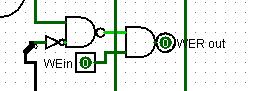
\includegraphics{MOV.png} \\
Figure 16: Write Enable 
\end{center}
\vspace{-.4cm}
\end{wrapfigure}
The final piece of the circuit deals with the MOVN and MOVZ commands. Since these two only write based on the given condition, we modify the write enable (WE in) if the condition was not met and the command was MOVN or MOVZ to begin with. In our implementation, the lower lead in to the NAND gate is the truth value of the condition, coming from the ALU (negated), and the upper lead in indicates whether or not the command is MOVN or MOVZ. As such, the output of the NAND gate is true if either the command is not MOVx, or if the condition was true. 

\subsection{Correctness Constraints}
The functional requirements for this circuit are as follows:
\begin{itemize}
\item The correctness of this module depends on the correctness of the inputs that are decoded in the Instruction Decode stage. Therefore, one functional requirement is that the inputs are consistent with the MIPS command given. For instance, WE in (write enable) must be 1 if the command ultimately writes back to the Register File. 
\item The module takes inputs from the Memory and Write Back Stages. Therefore, these stages need to be implemented correctly in order for this stage to be correct.
\item The execute subcircuit in this implementation is only correct for the instructions in Table A, and pseudo correct (set as NOPs) for the instructions in Table B. Only these instructions can be given in the Instruction Fetch Stage.

\end{itemize}

\subsection{Testing}
A large portion of the instructions depend on the correctness of the ALU circuit. Since that is given to us, we assume its correctness. For those instructions, computation is given correct, so we only have to test one case for each, that is, if one case gives us the correct nontrivial output (like 0 or something that could have been an accident), then the data path was correct and all inputs for that instruction should give us a correct output. \\

\noindent There are 6 functions that are not computed using the ALU: SLT, SLTU, SLTI, SLTIU, MOVN, and MOVZ. For these, we need to check an encompassing set of cases. Since all of these instructions involve a conditional, we check the cases for the conditionals, namely less than, greater than, and equal. \\ 

\noindent Lastly, we need to test the forwarding unit. We need to test for EX/MEM $\rightarrow$ EX forwarding and MEM/WB $\rightarrow$ EX forwarding. We test with multiple cases to be safe. 

\section{Memory}
The Memory Stage is not implemented for this Mini-MIPS project. However we do include a write enable bit and a multiplexor selector bit for the Memory. Aside from that, this stage is empty and only serves as a placeholder for Project 2. It also adds an extra clock cycle to the latency of the processor, though the throughput remains essentially the same. Data from this stage is also forwarded to the Execute Stage.\\
Testing is unnecessary as long as the multiplexor selector bit isn't on when it isn't supposed to be.

\section{Writeback}
The Writeback Stage only has one core functionality which is to store a value in a register if the write enable is 1. The only piece of circuit that isn't wiring in this Stage is the given Register File, so as long as our inputs are correct, there is no need to test this stage.

\section{Summary}
The design of \textbf{Project 1: Pipelined Mini-MIPS} consisted mainly of implementing the Decode and Execute stages and making the isolators to separate each section of the pipeline.  \\

\noindent In order to implement all of the operations required, we have to differentiate each one. We do this by creating more variables to pass through decode (in addition to the universally required variables such as \textbf{Write Enable}). For instance, because we have both signed comparison as well as unsigned comparison, the value \textbf{Signed} was created to differentiate the two. That value is passed into the Execute stage, which is then used as the select bit of a multiplexor. \\

\noindent After having all of the information required, we can begin executing the instruction. Since functionality of the the supplied ALU does not cover every operation, we have to add more pieces to our Execute stage. These pieces include a forwarding unit, comparators, and multiplexors for special outputs. \\

\noindent Once the Decode and Execute circuits have been created, the rest of the project was trivial. Isolators we created cleanly separate the different parts of the pipeline. The Instruction Fetch, Memory, and Writeback stages are all fairly simple, mostly consisting of connecting dots.\\

\noindent The skeleton of the pipeline has been created in this project. This will make Project 2, where Branches and Memory are introduced, much simpler. We will simply add to what is already there to make a more advanced processor.
\end{document}